%*******************************************************************************
% Preamble
%*******************************************************************************
% Instead of inserting \usepackage and defined commands here, they are in a separate file
% Queen's Thesis Format
% (Borrowed from Dean Jin's BigDis.tex file, then heavily modified :)

% Originally:
% Michelle L. Crane, Queen's University, 2003

% Then:
% Andrew W L Dickinson, Queen's University, 2011

% This revision:
% Kevin Hughes, Queen's University, 2013

%*******************************************************************************
% DOCUMENT STYLE
%*******************************************************************************
\documentclass[12pt]{report}
%-------------------------------------------------------------------------------------------------------------
\usepackage{quthesis}        % the Queen's University dissertation style file

%I don't even use the fancyheadings - it looks nice enough without it
%\usepackage{fancyheadings}  % doesn't seem to change the headings at all!
%*******************************************************************************


%*******************************************************************************
% SPACING
%*******************************************************************************
\usepackage{setspace}        % for use of \singlespacing and \doublespacing
%*******************************************************************************


%*******************************************************************************
% HEADINGS
%*******************************************************************************

% This changes the headings go that they are prettier, this can be commented out for traditional headings.
\usepackage{sectsty}
\allsectionsfont{\bfseries}% set all the section font to bfseries
\chapterfont{\centering\Large} % set the sizes of chapters, sections ...
\sectionfont{\normalsize}
\subsectionfont{\normalsize}

% for formatting Table of Contents entry, example: Chapter 1 Introduction
\usepackage[subfigure]{tocloft}
\usepackage{tocloft}
\renewcommand{\cftchappresnum}{Chapter }
\renewcommand{\cftchapaftersnum}{:}
\renewcommand{\cftchapnumwidth}{7em}

% for formatting Table of Contents entry for Appendix, example: Appendix 1: Stuff
\newcommand*\updatechaptername{%
   \addtocontents{toc}{\protect\renewcommand*\protect\cftchappresnum{Appendix }}
}

%*******************************************************************************
% FOOTNOTES
%*******************************************************************************

\interfootnotelinepenalty=10000 % This line stops footnotes from splitting onto two pages.

%*******************************************************************************
% VERBATIM
%*******************************************************************************
\usepackage{moreverb}        % Using this package to get better control of the
                             % verbatim environment, mostly for the use of the
                             % listing environment which puts line number
                             % beside each line.  Note that there has to be a number
                             % in each set of brackets, i.e., \begin{listing}[1]{1}.
                             % PDF info file is "The moreverb package" by
                             % Robin Fairbairns (rf@cl.cam.ac.uk) after
                             % Angus Duggan, Rainer Schopf and Victor Eijkhout, 2000/06/29.
%-------------------------------------------------------------------------------
%\usepackage{verbatim}        % allows the use of \begin{comment} and \end{comment}
                             % as well as \verbatiminput{file}
                             % Note:  when using verbatim to input from a text file,
                             % such as a specification or code, use \begin{singlespacing}
                             % and \end{singlespacing}.  Also, tabs are not read
                             % properly, so the input file must only use spaces.

%                             \begin{comment}
%                             Can also use the verbatim package for
%                             comments like this...
%                             \end{comment}
%*******************************************************************************


%*******************************************************************************
% GLOSSARY
%*******************************************************************************
\usepackage[nonumberlist]{glossaries}
\makeglossaries
\glossarystyle{list}
%*******************************************************************************


%*******************************************************************************
% LIST OF SYMBOLS
%*******************************************************************************
\usepackage{nomencl}
\makenomenclature
%*******************************************************************************


%*******************************************************************************
% INDEX
% Also possible to make an index; didn't use for my thesis.
%*******************************************************************************
\usepackage{makeidx}         % to make the index
\makeindex
%*******************************************************************************


%*******************************************************************************
% MATH STUFF
%*******************************************************************************
%-------------------------------------------------------------------------------
\usepackage{amsmath}         % to make nice equations
%-------------------------------------------------------------------------------
\usepackage{amsthm}          % to make nice theorem, i.e., definition

% Using the amsthm package, define a new theorem environment for my
% definition.  * means don't number it.
\newtheorem*{definition}{Definition}
%-------------------------------------------------------------------------------
\usepackage{cases}           % to make numbered cases (equations)
%-------------------------------------------------------------------------------
\usepackage{calc}            % Used with the Ventry environment defined below.
%*******************************************************************************


%*******************************************************************************
% FLOATS AND FIGURES
%*******************************************************************************
\usepackage{graphicx}        % for graphic images (use \includegraphics[...]{file.eps})
%-------------------------------------------------------------------------------
\usepackage{subfigure}       % for subfigures (figures within figures)
%-------------------------------------------------------------------------------
\usepackage{boxedminipage}   % to make boxed minipages, i.e., boxes around figures
%-------------------------------------------------------------------------------
\usepackage{rotate}          % for use of \begin{sideways} and \end{sideways}
%-------------------------------------------------------------------------------
\usepackage{listings}        % for use of printing code blocks
% Define how I would like the ``listings'' to look.
\lstset{basicstyle=\footnotesize,, numbers=left, numberstyle=\small, stepnumber=1, numbersep=5pt, showspaces=false, lineskip=-1pt}
%-------------------------------------------------------------------------------
\usepackage{float}           % Using this package to get better control of my floats
                             % including the ability to define new float types for
                             % my specification and code listings.
                             % DVI info file is "An Improved Environment for Floats"
                             % by Anselm Lingnau, lingnau@tm.informatik.uni=frankfurt.de
                             % 1995/03/29.

% Define new float styles here
% Ruled style for examples
%\floatstyle{ruled}
%\newfloat{Example}{h}{lop}[chapter]

% Style of float used for code listings
\floatstyle{ruled}
\newfloat{Listing}{H}{lis}[chapter]

                             % Note:  The listings don't have space between the chapters, unlike
                             % the standard list of tables etc.  At the end, copy the spacing
                             % commands from the .toc file and insert into the .lis file.  Then,
                             % DO NOT LATEX it again, simply go to the DVI viewer!

\usepackage{placeins} % for \FloatBarrier which stops floats from crossing a point
%*******************************************************************************
% TABLES
%*******************************************************************************
\usepackage{tabularx}        % Package used to make variable width-columns, i.e.,
                             % column widths are changed to fit the maximum width
                             % and text is wrapped nicely.

\usepackage{threeparttable}
%*******************************************************************************
% CAPTIONS
%*******************************************************************************
\usepackage[hang]{caption}   % Package used to make my captions 'hang', i.e., wrap
                             % around, but not under the name of the caption.
%-------------------------------------------------------------------------------------------------------------
% Find that the captions are too far from my verbatim figures, but if
% I change it to 0, then the captions are too close for my other types
% of figures.  Maybe set each one separately?
%\setlength{\abovecaptionskip}{1ex}

%\setlength{\textfloatsep}{1ex plus1pt minus1pt}

%\setlength{\intextsep}{1ex plus1pt minus1pt}

%\setlength{\floatsep}{1ex plus1pt minus1pt}
%*******************************************************************************


%*******************************************************************************
% MISCELLANEOUS
%*******************************************************************************
\usepackage{layout}          % useful for determining the margins of a document
                             % use with \layout command
%-------------------------------------------------------------------------------
\usepackage{changebar}       % Way of indicating modifications by putting bars in the
                             % margin.  Read about it in "The Latex Companion".
%-------------------------------------------------------------------------------
%\usepackage{ccfonts,eulervm} 	% fonts I like from Knuth's "Concrete Mathematics"
%\usepackage[T1]{fontenc}
%*******************************************************************************

%*******************************************************************************
% REFERENCES ETC.
%*******************************************************************************
\usepackage{varioref}        % Better page references, e.g., "on preceding page", etc.
                             % \vref{key} Create an enhanced reference.
                             % \vpageref[text]{key} Create an enhanced page reference.
                             % \vrefrange{key}{key} Create an enhanced range of references.
                             % \vpagerefrange[text]{key}{key} Create an enhanced range of page references.
                             % Note: doesn't really work for consecutive pages.

% Renewing the text for before and after, because I don't like the default flip-flopping one.
% And 'on the page before' sounds dumb!

\renewcommand{\reftextafter}{on the next page}
\renewcommand{\reftextbefore}{on the previous page}
%-------------------------------------------------------------------------------
\usepackage{url}             % for use of \url - pretty web addresses
\usepackage{fancyhdr}
\usepackage{cite}

%*******************************************************************************
% HYPERLINKS (must be last)
%*******************************************************************************

% Uncomment these next two lines for linkback to citation pages in biblio
% \renewcommand*\backref[1]{\ifx#1\relax \else \linebreak Cited on page(s): #1. \fi}

\usepackage[bookmarks,pdfauthor={Kevin Andrew Hughes}, pdftitle={Thesis Title}]{hyperref}

\hypersetup{colorlinks=true,  % Change links to being coloured text, no boxes
		linkcolor=blue,
}
                             % Neat package to turn href, ref, cite, gloss entries
                             % into hyperlinks in the dvi file.
                             % Make sure this is the last package loaded.
                             % Use with dvips option to get hyperlinks to work in ps and pdf
                             % files.  Unfortunately, then they don't work in the dvi file!
                             % Use without the dvips option to get the links to work in the dvi file.

                             % Note:  \floatstyle{ruled} don't work properly; so change to plain.
                             % Not as pretty, but functional...
                             % The bookmarks option sets up proper bookmarks in the pdf file :)

% Need this command to allow hyperref to play nicely with gloss; otherwise
% almost every \gloss will cause an error...
%\renewcommand{\glosslinkborder}{0 0 0}
%*******************************************************************************


%*******************************************************************************
% MISCELLANEOUS COMMANDS AND ENVIRONMENTS
%*******************************************************************************
% Use this command to show more table of contents - used when playing
% with the draft outline
% I think it should be about 2???
\setcounter{tocdepth}{2}
%*******************************************************************************
% Environment definition I found in the "The Latex Companion".  Used to
% create a list environment where the indenting is the same for all of the
% entries, regardless of their length.  Note:  must \usepackage{calc}.
\newenvironment{Ventry}[1]%
    {\begin{list}{}{\renewcommand{\makelabel}[1]{\textbf{##1}\hfil}%
        \settowidth{\labelwidth}{\textbf{#1:}}%
        \setlength{\leftmargin}{\labelwidth+\labelsep}}}%
    {\end{list}}
%*******************************************************************************

%*******************************************************************************
% MY DEFINED COMMANDS
%*******************************************************************************
% Command that I can use to create notes in the margins;
% adapted from Juergen's META tag
%\newcommand{\meta}[1]{\begin{singlespacing}
%{\marginpar{\emph{\footnotesize Note: #1}}}\end{singlespacing}}
%*******************************************************************************
% Command that I can use to create lined headings
%\newcommand{\heading}[1]{\bigskip \hrule \smallskip \noindent \texttt{#1} \smallskip \hrule}
%*******************************************************************************
% Command that I can use for reading in a file, verbatim, with line
% numbers printed along the left side.  The parameter is the file name.
%\newcommand{\fileinnum}[1]{
%    \begin{singlespacing} {\footnotesize
%    \begin{listinginput}[1]{1}{#1}\end{listinginput}
%    }\end{singlespacing}
%}
%*******************************************************************************
% Command that I can use for reading in a file, verbatim, with NO line
% numbers, but in a smaller font.  The parameter is the file name.
\newcommand{\filein}[1]{
   \begin{singlespacing}{\footnotesize
    \begin{verbatiminput}{#1}\end{verbatiminput}
    }\end{singlespacing}
}
%*******************************************************************************
% Command that I can use for reading in a file, verbatim, with NO line
% numbers, but in a smaller font.  The parameter is the file name.
\newcommand{\fileinsmall}[1]{
    \begin{singlespacing}{\scriptsize
    \begin{verbatiminput}{#1}\end{verbatiminput}
    }\end{singlespacing}
}
%*******************************************************************************
% Dean't 'notesbox' command.  Needs setspace package.
%   Usage: \notesbox{This is a note.}
%%
\usepackage{setspace}
\newcommand{\notesbox}[1]{
     \begin{singlespacing}
      \noindent\begin{boxedminipage}[f]{\textwidth}{\sf{#1}}\end{boxedminipage}
	\vspace{-24pt}
     \end{singlespacing}
}


% Change the author name and pdf title in the preamble line 235

%*******************************************************************************
% DOCUMENT
%*******************************************************************************

\begin{document}

%*******************************************************************************
% TITLE
%*******************************************************************************

\title{Thesis Title}

\author{Kevin Hughes}

\dept{Faculty of Electrical and Computer Engineering}
\degree{Master of Applied Science}

% ~~~~~~~~~~~~~
%\submitdate{June 2013}
%        - date LaTeX'd if omitted
%\copyrightyear{2013}
%        - year LaTeX'd if omitted

\beforepreface

%*******************************************************************************
% ABSTRACT
%*******************************************************************************

\prefacesection{Abstract}
Abstract

%*******************************************************************************
% ACKNOWLEDGEMENTS
%*******************************************************************************

\phantomsection
\prefacesection{Acknowledgements}
Acknowledge some people here

\clearpage % keep this for proper page numbering!

%*******************************************************************************
% STATEMENT OF ORIGINALITY (required CHEM, CISC, GEOL, MATH, PHYS (Ph.D. only))
%*******************************************************************************

%\phantomsection
%Statement of Originality goes here if required
%\clearpage

%*******************************************************************************
% Table of Contents
%*******************************************************************************
% The Table of Contents and the following sections up until the main chapters are generated
% by code in the quthesis.sty file particularly \def\afterpreface... around line 248

%*******************************************************************************
% Glossary
%*******************************************************************************
% make sure Glossary Packages etc. are uncommented in 0_Preamble.tex
\glosspagetrue
\newacronym{AI}{AI}{Artificial Intelligence}

\newglossaryentry{OpenCV}{
	name={OpenCV},
	description={Open source Computer Vision library for C++\cite{opencv}}
}

\glsaddall


%*******************************************************************************
% List of Symbols
%*******************************************************************************
% make sure List of Symbols Packages etc. are uncommented in 0_Preamble.tex
\symbolspagetrue

%*******************************************************************************
% List of Figures
%*******************************************************************************
\figurespagetrue

%*******************************************************************************
% List of Code Listings
%*******************************************************************************
\listingspagetrue

%*******************************************************************************
% List of Tables
%*******************************************************************************
\tablespagetrue

%*******************************************************************************
% CHAPTERS
%*******************************************************************************
\singlespacing \afterpreface \doublespacing

% This command can be used to view the page layout for this document
% \layout

% Here, I'm tweaking how much space is put above and below floats.
% Comment out if you want the *purest* latex spacing.
%\setlength{\abovedisplayskip}{3pt plus1pt minus1pt}
%\setlength{\abovedisplayshortskip}{3pt plus1pt minus1pt}
%\setlength{\belowdisplayskip}{3pt plus1pt minus1pt}
%\setlength{\belowdisplayshortskip}{3pt plus1pt minus1pt}


% Include chapters - kept separated to make editing easier.
% Chapter 1
\glsresetall % reset the glossary to expand acronyms again
\chapter{Introduction}\label{ch:Introduction}

% Motivation
\section{Motivation}
Motivation


% Problem Overview
\section{Problem Overview}
Problem Overview


% Thesis Contributions
\section{Thesis Contributions}

The main contributions of this thesis are as follows:

\begin{itemize}
\item{Contribution 1}
\item{Contribution 2}
\item{Contribution 3}
\item{...}
\end{itemize}


% Thesis Outline
\section{Thesis Outline}
The remainder of this thesis is organized as follows:

\noindent\textbf{Chapter 2, Background:} Background

\noindent\textbf{Chapter 3, Methods:} Methods

\noindent\textbf{Chapter 4, Results:} Results

\noindent\textbf{Chapter 5, Conclusions and Future Work:} Conclusions

% Chapter 2
\glsresetall % reset the glossary to expand acronyms again
\chapter{Background}\label{ch:Background}
Background

% Sections
\section{Examples}
text
\subsection{Sub Section}
text
\subsubsection{Sub Sub Section}
text

% Example Glossary
\noindent \gls{AI}

% Example Reference
\noindent thanks to OpenCV\cite{opencv}

% Example Figure
% reference this figure in the text using \ref{fig.testPlot}
\begin{figure}[!htbp]
	\centering
	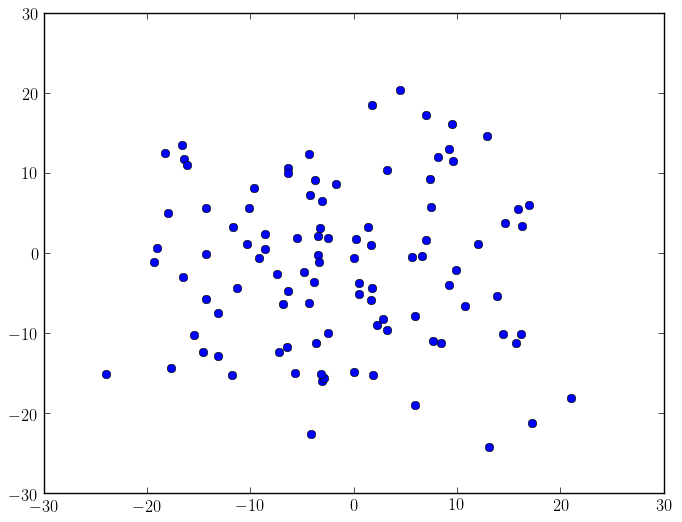
\includegraphics[width = 5in]{figs/testPlot.png}
	\caption{Test Plot}
	\label{fig.testPlot}
\end{figure}

% Example Equation
% I recommend using http://www.codecogs.com/latex/eqneditor.php to help make equations
% for tough equations or until you're familiar with LaTeX
% reference in the text using \ref{eqn.lowpassfilter}
\begin{equation}
	\mu_t = \alpha x + (1 - \alpha) \mu_{t-1}
	\label{eqn.lowpassfilter}
\end{equation}

% Example Nomenclature
\nomenclature{$\mu$}{Average}

% Example Code Listing
% reference in the text using \ref{ls.testPlot}
\lstset{language=python}
\lstset{tabsize=4}
\lstset{commentstyle=\color{blue}}
\lstset{frame=single}
\lstset{label = ls.testPlot}
\lstset{caption = Test Plot Code }
\lstinputlisting[float=!htbp]{figs/testPlot.py}

% Example Table
% I recommend using http://truben.no/latex/table/ to help with making tables
% reference in the text using \ref{tab.testTable}
\begin{table}[!htbp]
    \centering
    \begin{tabular}{|l|l|l|} % options are l,c,r (left, center, right)
    \hline
    ~ & ~ & ~ \\
    \hline
    ~ & ~ & ~ \\
    \hline
    ~ & ~ & ~ \\
    \hline
    ~ & ~ & ~ \\
    \hline
    \end{tabular}
    \caption{Test Table}
    \label{tab.testTable}
\end{table}

% Chapter 3
\glsresetall % reset the glossary to expand acronyms again
\chapter{Methods}\label{ch:Methods}
Methods

% Chapter 4
\glsresetall % reset the glossary to expand acronyms again
\chapter{Results}\label{ch:Results}
Results

% Chapter 5
\glsresetall % reset the glossary to expand acronyms again
\chapter{Conclusions and Future Work}\label{ch:Conclusion}

\section{Summary of Conclusions}
Conclusions

\section{Future Work}\label{sec:FutureWork}
Future Work


%*******************************************************************************
% BIBLIOGRAPHY
%*******************************************************************************

% Put in \nocite{*} so all entries in the bibliography are included
% \nocite{*}

\phantomsection
\bibliographystyle{plain}
\bibliography{references/references}

%*******************************************************************************
% APPENDICES
%*******************************************************************************
%\updatechaptername
%\appendixpage
%\appendix

%\include{6_Appendices}

%*******************************************************************************
% INDEX
%*******************************************************************************
% Here's where the index would be printed, if you created one.  Default: no.
% Remove the % on the next line to enable.
%\printindex


%********************t***********************************************************
% End DOCUMENT
%*******************************************************************************
\end{document}
